\documentclass[10pt,pdf,utf8,russian,aspectratio=169]{beamer}
\usepackage[T2A]{fontenc}
\usepackage[english,russian]{babel}
\usepackage{float}
\usepackage[normalem]{ulem}

\usetheme{metropolis}   

\usepackage{booktabs}
\usepackage[scale=2]{ccicons}


\usepackage{pgfplots}
\usepgfplotslibrary{dateplot}

\definecolor{BI}{RGB}{63,143,213}
\setbeamercolor{frametitle}{bg=BI}
\setbeamercolor{title separator}{fg=BI}
\setbeamercolor{progress bar in section page}{fg=BI}

\title{GeneQuery}
\subtitle{Система поиска фенотипов}
\date{\today}
\author{Арбузов Иван}
\institute{Институт Биоинформатики}
\titlegraphic{\hfill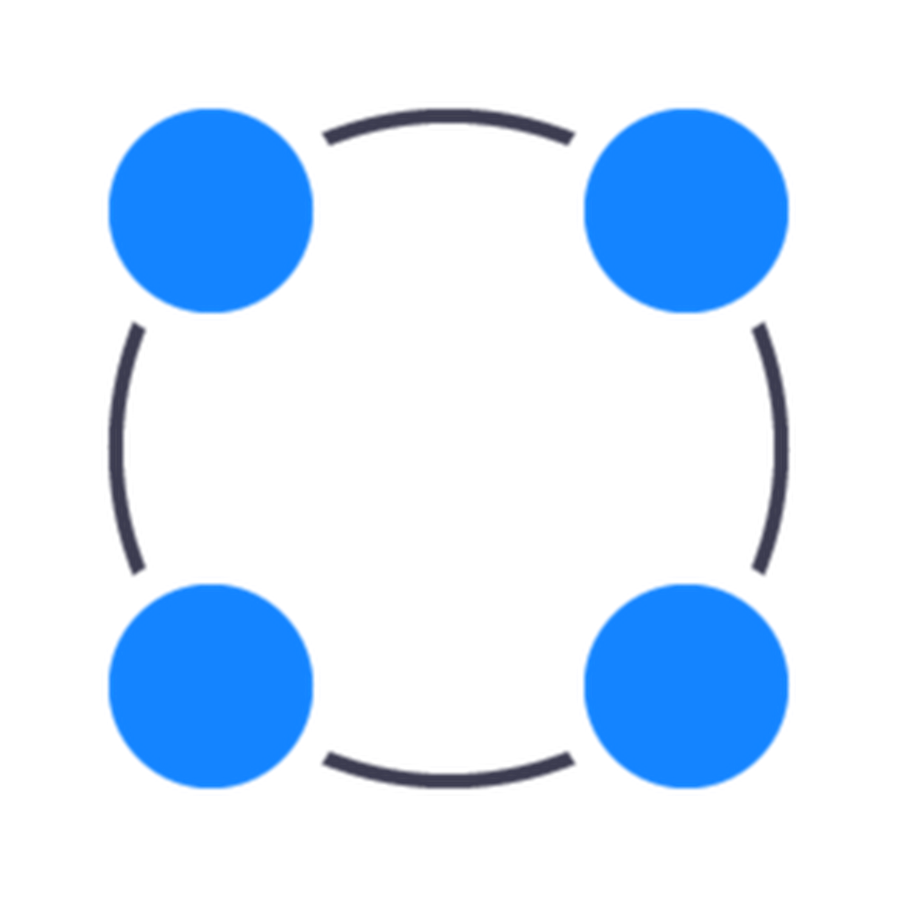
\includegraphics[height=1.5cm]{logo}}

\begin{document}

\maketitle

\begin{frame}
  \frametitle{Содержание}
  \setbeamertemplate{section in toc}[sections numbered]
  \tableofcontents
\end{frame}

\section{Введение в поиск фенотипов}

\begin{frame}{Описание проблемы}
  \begin{itemize}[<+->]
    \item Провели эксперемент
    \item Получили набор «проявивших» себя генов
    \item \alert{Как проинтерпретировать результат?}
  \end{itemize}
\end{frame}

\begin{frame}{Интерпретация результата}
  \begin{itemize}[<+->]
    \item Экспертная интерпретация
    \item Лексический анализ (текстов, статей и т.д.)
    \item \alert<4> {Аналитическая интерпретация (статистика, теория вероятностей и т.д.)}
  \end{itemize}
\end{frame}

\begin{frame}{Общая постановка задачи}
  \begin{itemize}[<+->]
    \item Имеется множество результатов (наборов одинаково регулируемых генов) уже проделанных экспериментов
    \item Имеется результат (набор генов) нового эксперимента
    \item Найти среди уже сделанных экспериментов те, в которых гены ведут себя \alert<4>{«похожим»} образом
  \end{itemize}
\end{frame}


\section{GeneQuery: обзор}

\begin{frame}{Используемые данные}
  \begin{itemize}[<+->]
    \item Основан на базе данных GEO
    \item Датасет содержит информацию об экспрессии генов $k$ фенотипов, участвовавших в эксперименте
    \item 6000 наиболее «активных» генов разбиты на кластеры алгоритмом WGCNA
    \item Pathway экспрессий генов одного кластера \emph{совпадает} (up-/down-regulated)  
    \item $\sim$ 50k кластеров для мышки, $\sim$ 80k --- для человека
  \end{itemize}
\end{frame}

\begin{frame}{Архитектура}
    \begin{figure}[p]
        \centering
        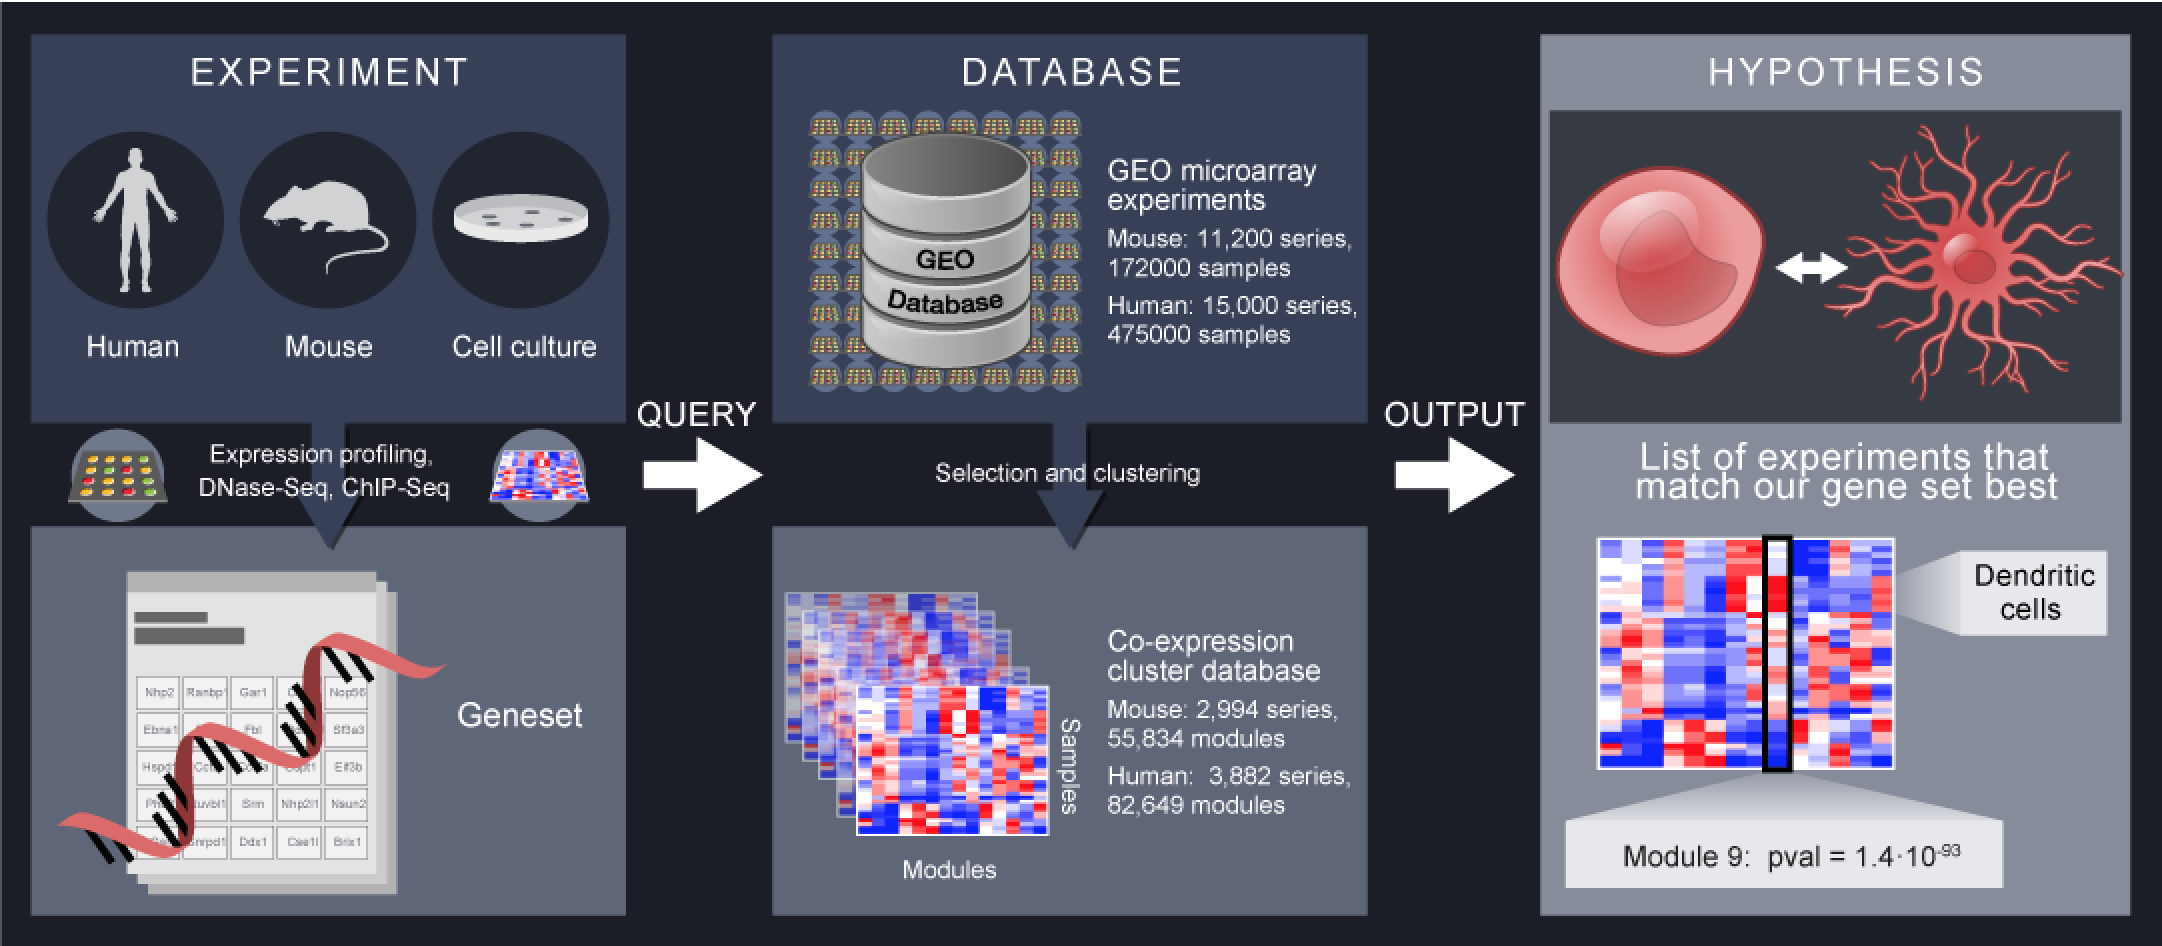
\includegraphics[width=0.9\textwidth]{./img/architecture.png}
    \end{figure}      
\end{frame}

\begin{frame}
    \begin{figure}[p]
        \centering
        \caption{Форма запроса.}
        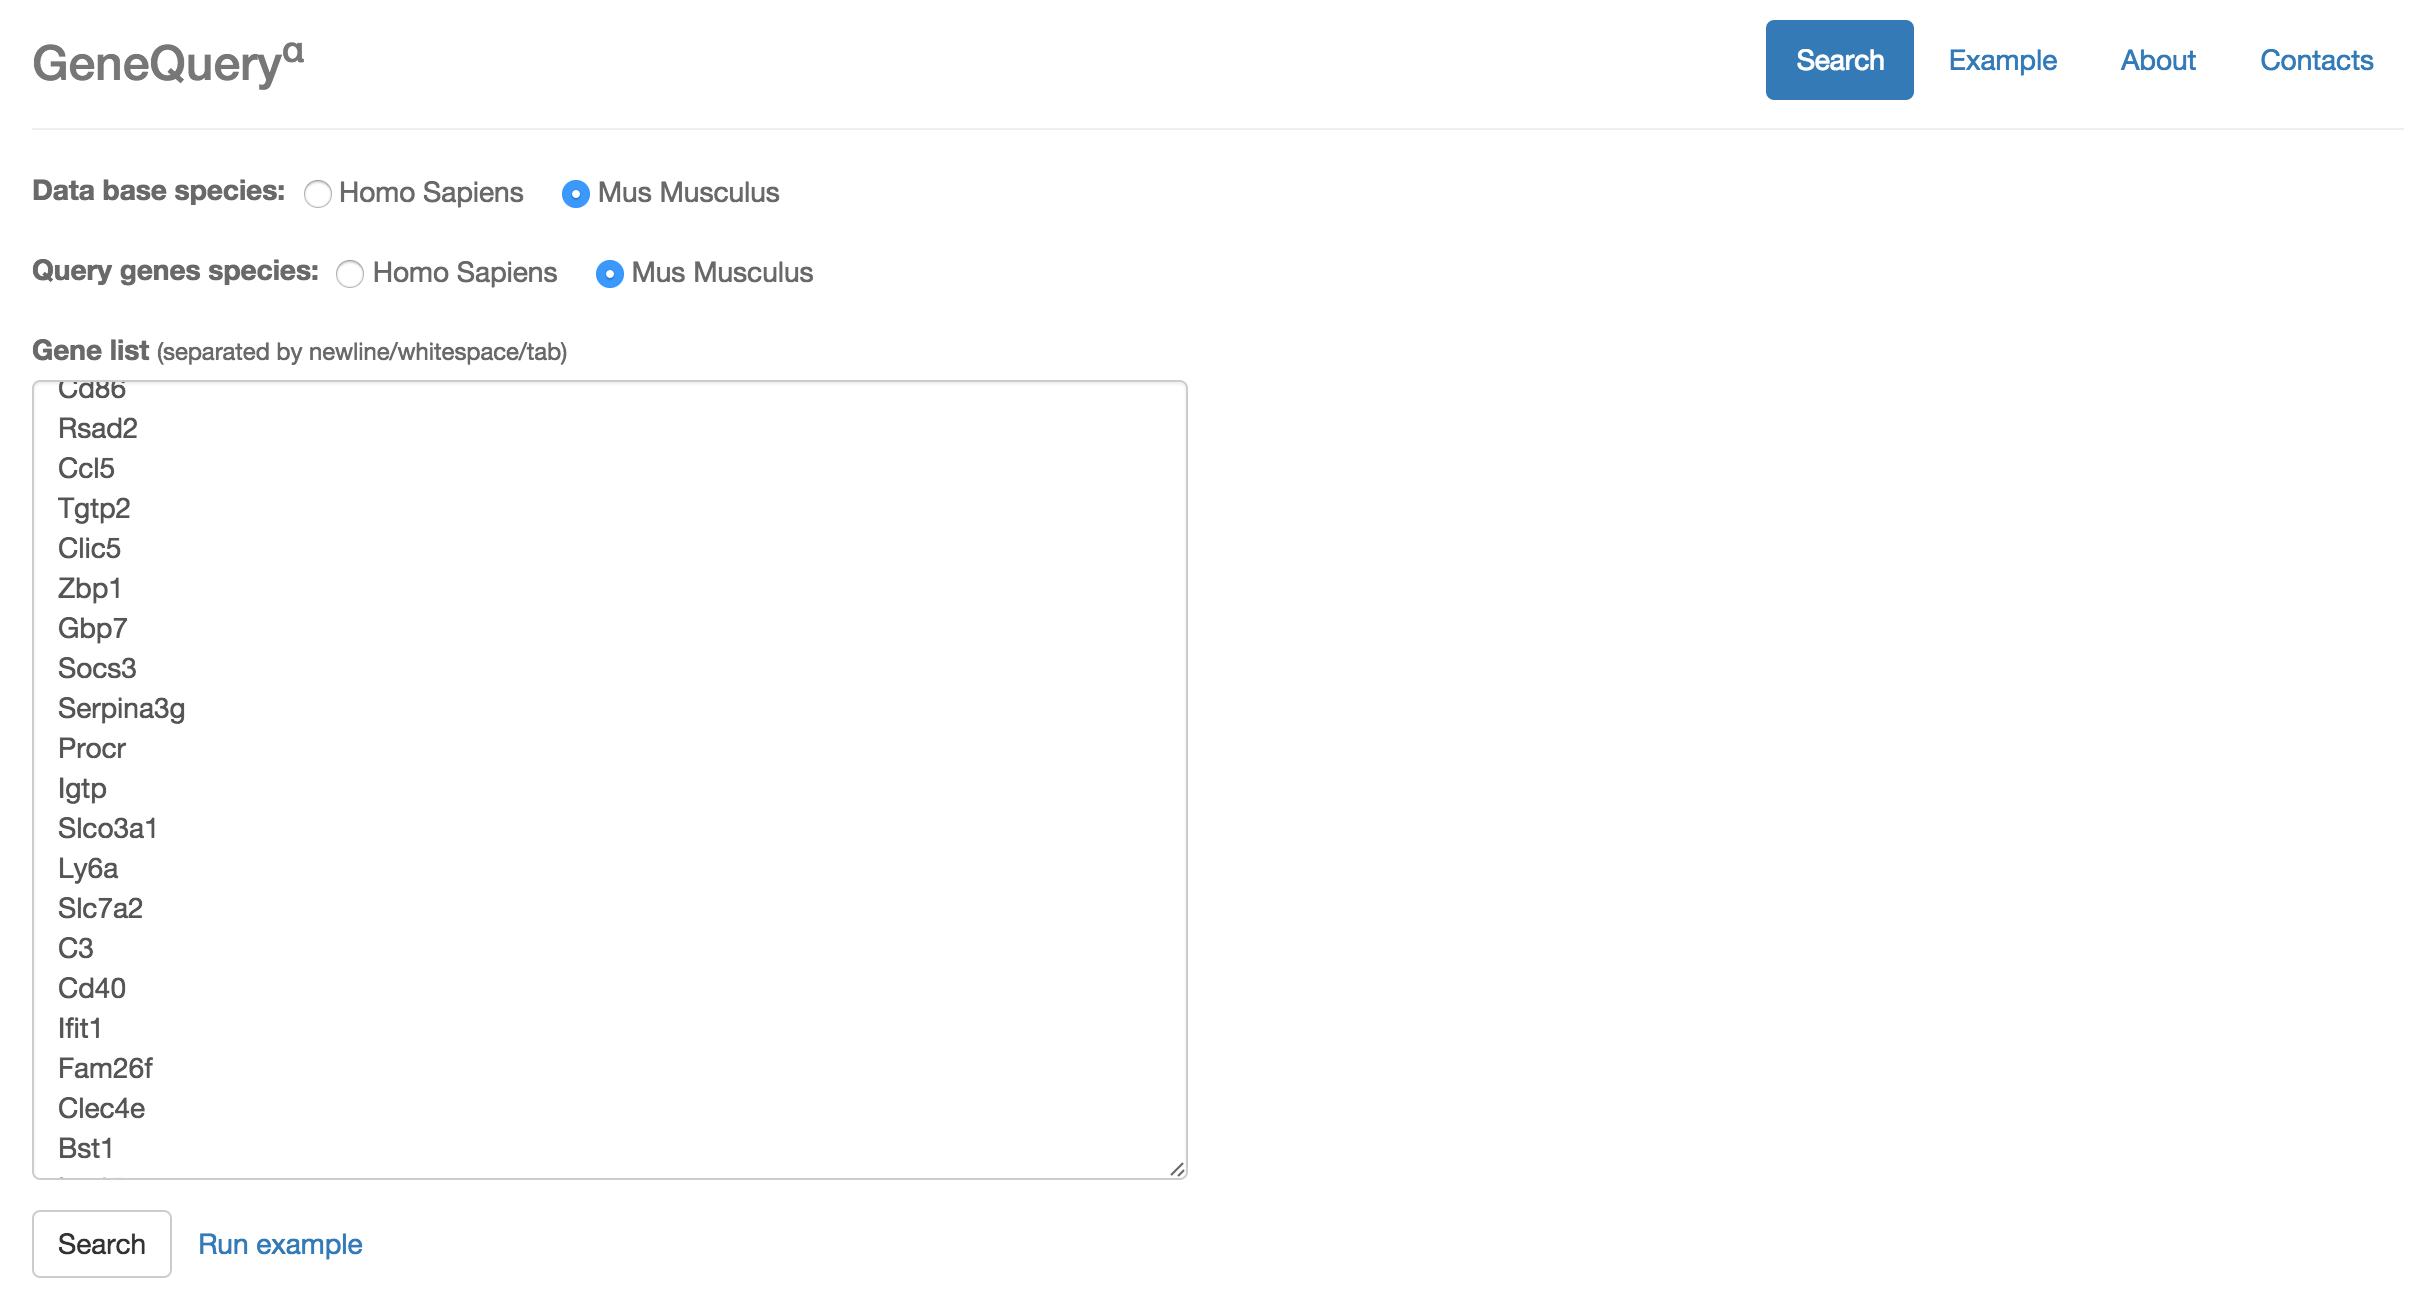
\includegraphics[height=0.9\textheight]{./img/screen_query.png}
    \end{figure}
\end{frame}

\begin{frame}
    \begin{figure}[p]
        \centering
        \caption{Таблица с результатами.}
        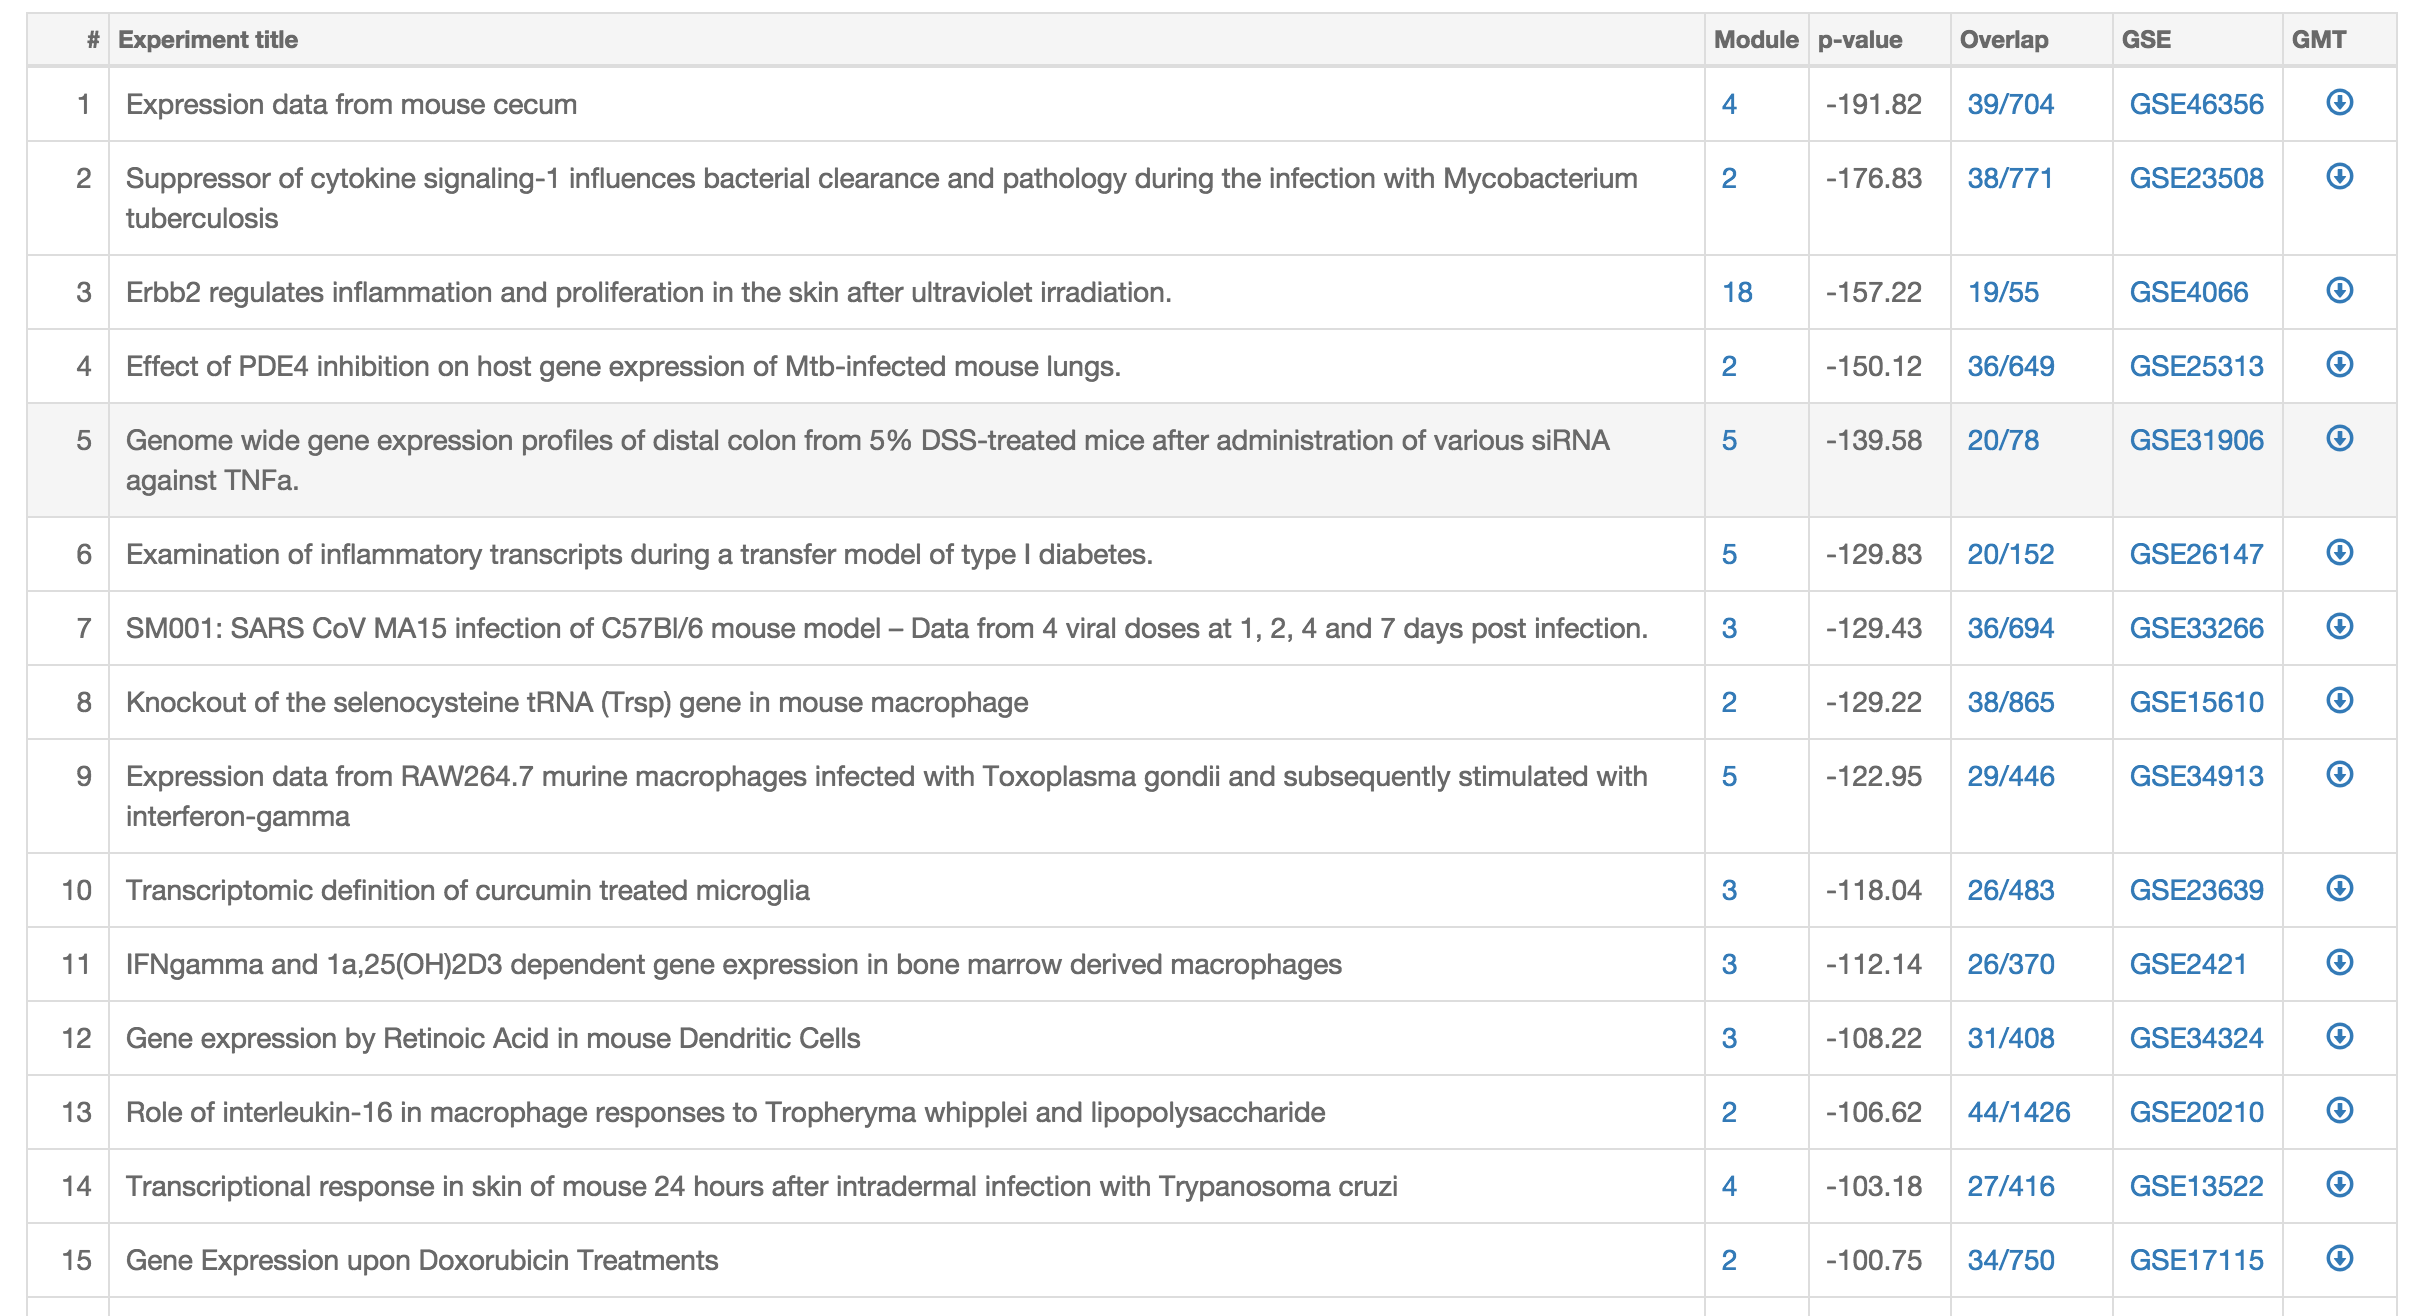
\includegraphics[height=0.9\textheight]{./img/screen_results.png}
    \end{figure}
\end{frame}

\begin{frame}
    \begin{figure}[p]
        \centering
        \caption{Детализация конвертации генов.}
        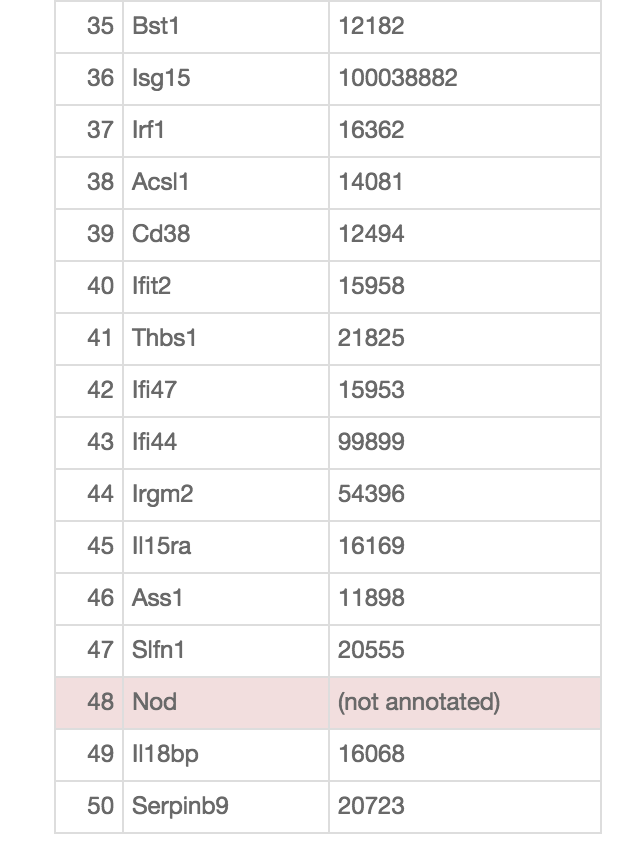
\includegraphics[height=0.9\textheight]{./img/screen_details.png}
    \end{figure}
\end{frame}

\begin{frame}
    \begin{figure}[p]
        \centering
        \caption{Heatmap.}
        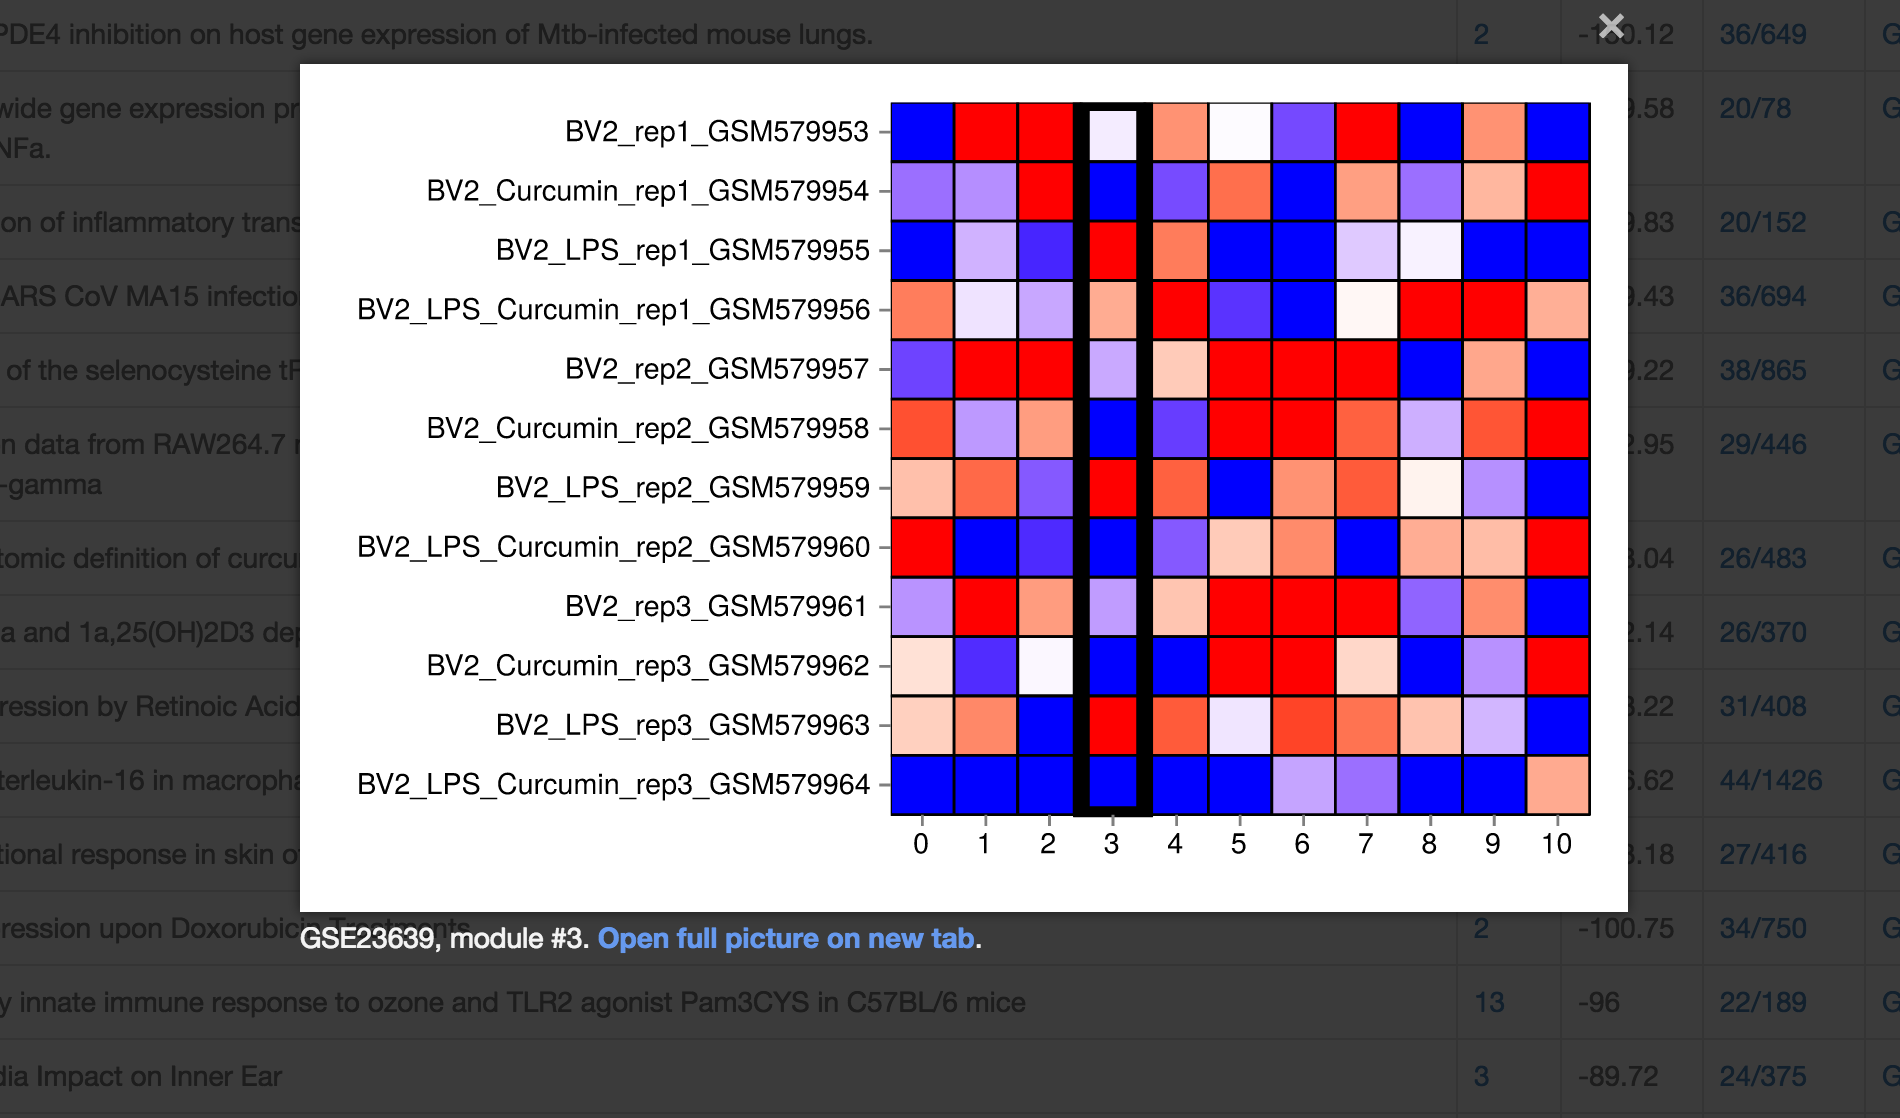
\includegraphics[height=0.9\textheight]{./img/screen_heat.png}
    \end{figure}
\end{frame}

\begin{frame}
    \begin{figure}[p]
        \centering
        \caption{Гены из пересечения в Symbol нотации.}
        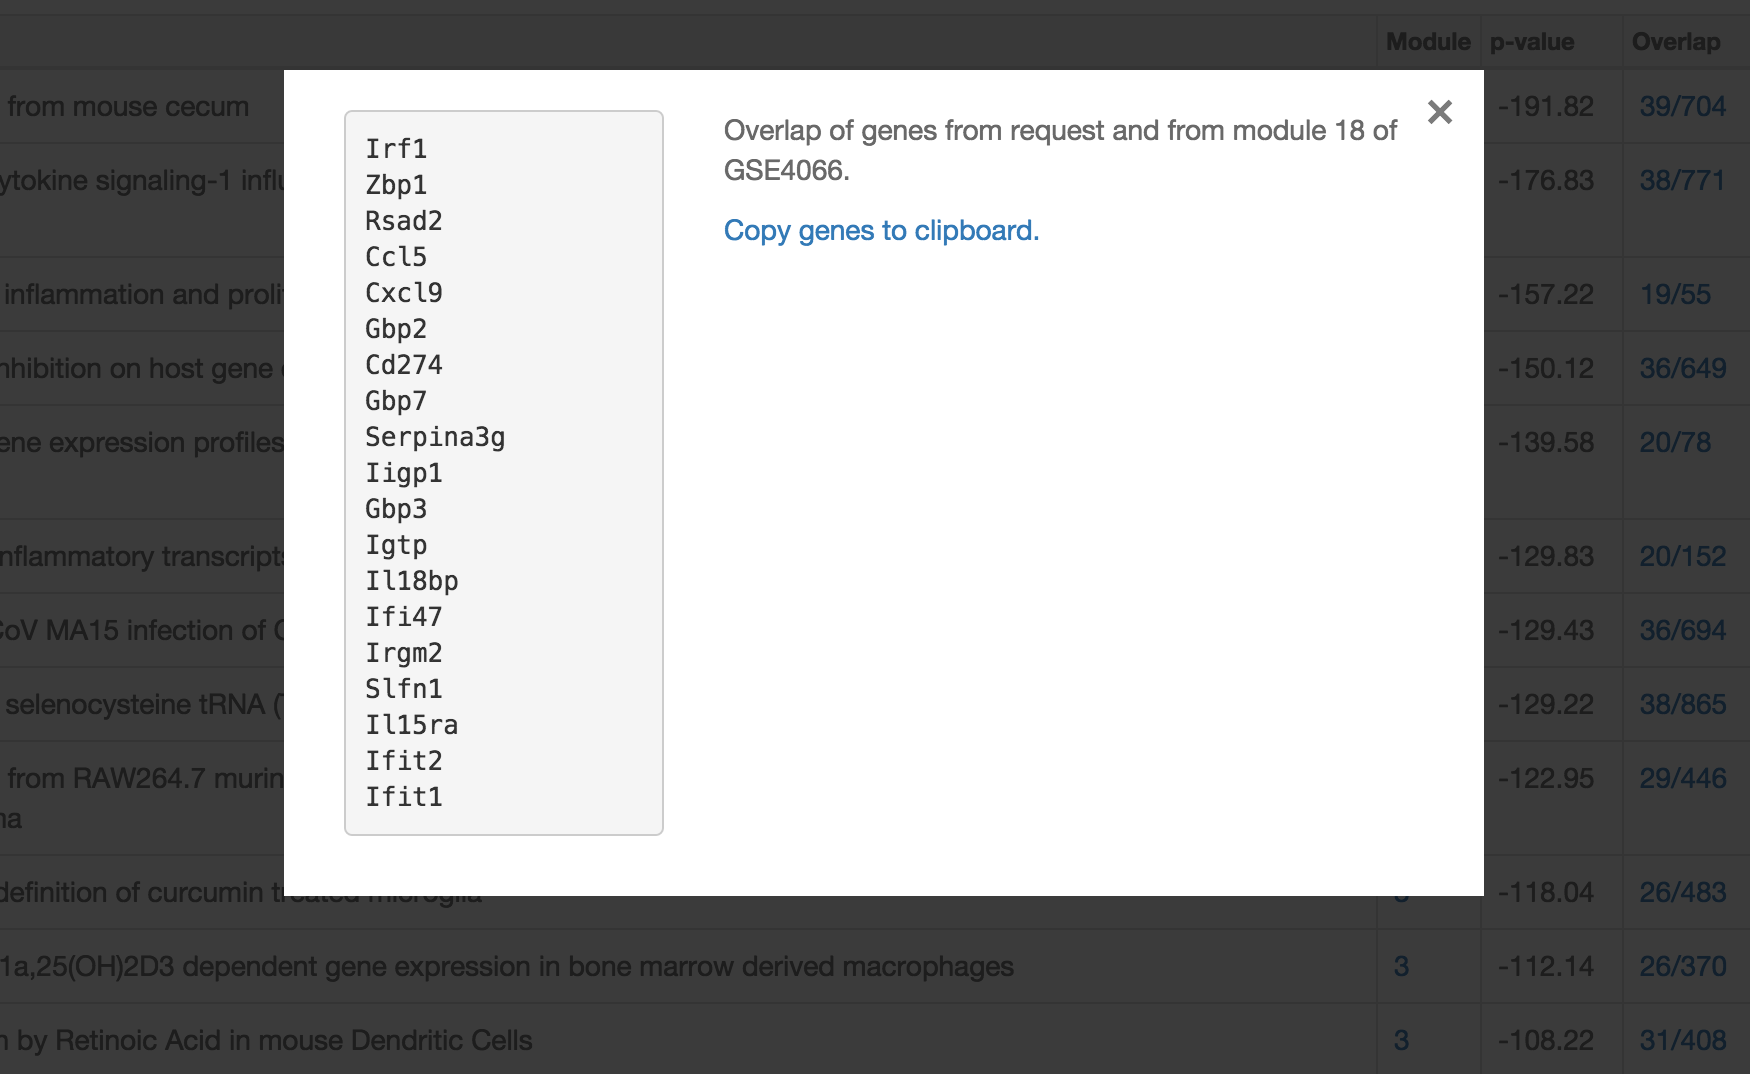
\includegraphics[height=0.9\textheight]{./img/screen_overlap.png}
    \end{figure}
\end{frame}


\section{GeneQuery: под капотом}

\subsection{Вероятностная модель}

\begin{frame}{Условности}
  \begin{itemize}[<+->]
    \item Ген уникально идентифицируется своим \emph{Entrez ID} --- неким натуральным числом
    \item Запрос --- набор генов ненулевого размера
    \item Модуль --- кластер после работы алгоритма WGCNA
    \item GSE --- все кластеры какого-либо эксперимента (с $k$ фенотипами)
  \end{itemize}
\end{frame}

\begin{frame}{Пересечение запроса и модуля}
  \begin{itemize}[<+->]
    \item Пусть имеется некоторый набор генов (запрос)
    \item Зафиксируем какой-либо модуль из нашей базы данных
    \item Найдем пересечение запроса и модуля
    \item \emph{Какова вероятность получить получить именно такое пересечение?}
    \item Гипергеометрическое распределение
  \end{itemize}
\end{frame}

\begin{frame}{Понимаем гипергеометрическое распределение}
  \begin{itemize}[<+->]
    \item Пусть имеется урна с $N$ шариками двух цветов: $D$ белых, $N - D$ черных
    \item Вытянем из урны $n$ шаров одновременно
    \item Какова вероятность, что $k$ из $n$ шаров окажутся белыми?
  \end{itemize}
\end{frame}

\begin{frame}{Точная формула вероятности}
    \begin{block}{Вероятность вытянуть $k$ белых шаров}
        \begin{equation}
        f(k; N, D, n) = \frac{\binom{D}{k}\binom{N - D}{n - k}}{\binom{N}{n}}
        \end{equation},
        где $N$ --- шаров в урне,
            $D$ --- белых шаров в урне,
            $n$ --- количество вытянутых шаров,
            $k$ --- количество вытянутых \emph{белых} шаров.
    \end{block}
\end{frame}

\begin{frame}{Сведение к гипергеометрическому распределению}
  \begin{itemize}[<+->]
    \item Пусть $N$ --- множество всех генов GSE ($\sim 6000$), $D$ --- множество генов в запросе
    \item «Покрасим» в белый цвет те гены из $N$, которые присутствуют и в $D$
    \item Пусть $n$ --- какой-либо модуль из данного GSE
    \item \emph{Какова вероятность, что $k$ генов из этого модуля «покрашены» в белый цвет, т.е. принадлежат множеству генов из запроса?}
  \end{itemize}
\end{frame}

\begin{frame}{Точная формула вероятности}
    \begin{block}{Вероятность иметь $k$ генов из запроса в модуле $n$}
        \begin{equation}
        f(k; N, D, n) = \frac{\binom{D}{k}\binom{N - D}{n - k}}{\binom{N}{n}}
        \end{equation},
        где $N$ --- количество генов в GSE, которому принадлежит модуль $n$,
            $D$ --- количество генов в запросе,
            $n$ --- количество генов в модуле,
            $k$ --- количество генов в пересечении модуля и запроса.
    \end{block}
\end{frame}

\begin{frame}{Оценка значимости пересечения}
  \begin{itemize}[<+->]
    \item На сколько данное пересечение статистически значимо?
    \item Точный тест Фишера
  \end{itemize}
\end{frame}

\begin{frame}{Точный тест Фишера}
    Рассмотрим таблицу
    \begin{table}[!ht]
        \centering
        \begin{tabular}{c|c|c|c}
                 & Юноши   & Девушки &  Всего \\ \hline
        на диете & $a$     & $b$     & $a + b$ \\ \hline
     не на диете & $c$     & $d$     & $c + d$ \\ \hline
           всего & $a + c$ & $b + d$ & $n$ \\
        \end{tabular}
    \end{table}
    Вероятность того, что $a$ юношей не на диете, вычисляется по формуле гипергеометрического распределения:
        $$\mathsf{Pr}(a) = \frac{\binom{a + b}{a}\binom{c + d}{c}}{\binom{n}{a + c}}$$
\end{frame}

\begin{frame}{Точный тест Фишера: пример}
    Рассмотрим таблицу
    \begin{table}[!ht]
        \centering
        \begin{tabular}{c|c|c|c}
                 & Юноши   & Девушки &  Всего \\ \hline
        на диете & $1$     & $9$     & $10$ \\ \hline
     не на диете & $11$     & $3$     & $14$ \\ \hline
           всего & $12$ & $12$ & $24$ \\
        \end{tabular}
    \end{table}
    \onslide<2->{Какова вероятность, что из 12 юношей лишь один будет на диете?} \\
    \onslide<3>{Правда ли, что склонность к диете не зависит от пола?}
\end{frame}

\begin{frame}{Точный тест Фишера}
  \begin{itemize}[<+->]
    \item Нулевая гипотеза: \emph{склонность к диете не зависит от пола}
    \item Посчитаем вероятность получить такое или более \emph{«перекошенное»} (при одинаковой сумме в строках и столбцах) распределение юношей
    \item Эта вероятность --- статистическая значимость наблюдения
  \end{itemize}
\end{frame}

\begin{frame}{Точный тест Фишера: пример}
    В нашем примере только одна таблица более перекошена:
    \begin{table}[!ht]
        \centering
        \begin{tabular}{c|c|c|c}
                 & Юноши   & Девушки &  Всего \\ \hline
        на диете & $0$     & $10$     & $10$ \\ \hline
     не на диете & $12$     & $2$     & $14$ \\ \hline
           всего & $12$ & $12$ & $24$ \\
        \end{tabular}
    \end{table}
    \onslide<2->{
        Результирующая значимость будет вычисляться:
        $$p_{value} = \mathsf{Pr}(1) + \mathsf{Pr}(0)$$
    }
    \onslide<3->\emph{
        При выполнении нулевой гипотезы вероятность получить исходную таблицу равна $p_{value}$
    }
\end{frame}

\begin{frame}{Применение теста Фишера}
    Для оценки статистической значимости пересечения запроса с модулем используется таблица:
     \begin{table}[!ht]
        \centering
        \begin{tabular}{c|c|c|c}
                 & пересек. с GSE & не пересек.с GSE & Всего \\  \hline
        в модуле & $k$            & $n - k$          & $n$ \\ \hline
     не в модуле & $D - k$        & $N - D + k - n$  & $N - n$ \\ \hline
           всего & $D$            & $N - D$          & $N$ \\
        \end{tabular}
    \end{table}
    \onslide<2->{
        Результирующая значимость получается по формуле:  
        $$ p_{value} = \sum_{i = k}^{min(D, n)} \mathsf{Pr}(i) $$
        т.н. \emph{правосторонний} тест Фишера.
    }
\end{frame}

\begin{frame}{Проблема множественных сравнений}
  \begin{itemize}[<+->]
    \item Статистический тест дает точный результат при \emph{одном} испытании
    \item При увеличении количества испытаний вероятность \emph{случайно} получить низкий $p_{value}$ (т.е. значимый результ) возрастает
    \item Поправка Бонферрони решает проблему, но грубо:
    $$\hat{p_i} = p_i \times m$$, где $m$ --- количество испытаний, $p_i$ --- значимость результата $i$-го испытания, $\hat{p_i}$ --- новоя значимость
  \end{itemize}
\end{frame}

\subsection{Bootstrapping}

\begin{frame}{Множественные сравнения в GeneQuery}
  \begin{itemize}[<+->]
    \item Рассмотрим, как устроены данные в GeneQuery
    \item Далее под $p_{value}$ понимается минимальное $p_{value}$ среди всех модулей для конкретного вида (человек или мышь)
  \end{itemize}
\end{frame}
   
   
\begin{frame}
    \begin{figure}[p]
        \centering
        \caption{Распределение $log(p_{value})$ для запросов из 500 генов. Человек.}
        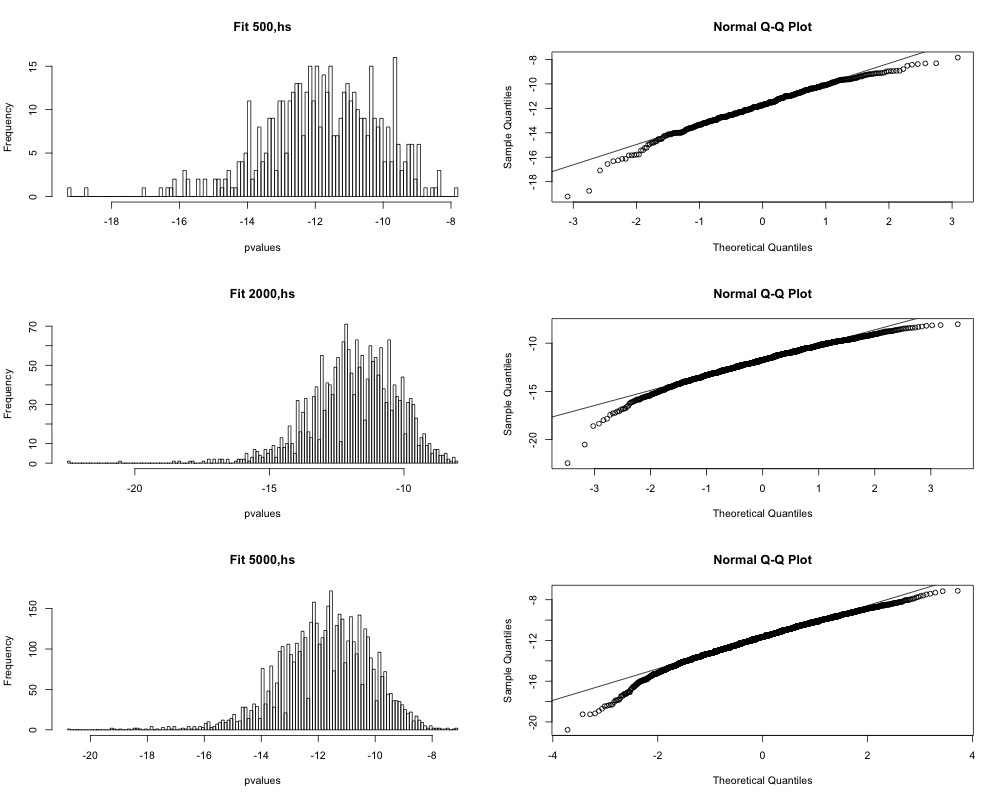
\includegraphics[height=0.95\textheight]{./img/converge_to_norm_query_size_500_hs.jpeg}
    \end{figure}
\end{frame}

\begin{frame}
    \begin{figure}[!ht]
        \centering
        \caption{Распределение $log(p_{value})$ для запросов из 25, 250, 2500 генов.}
        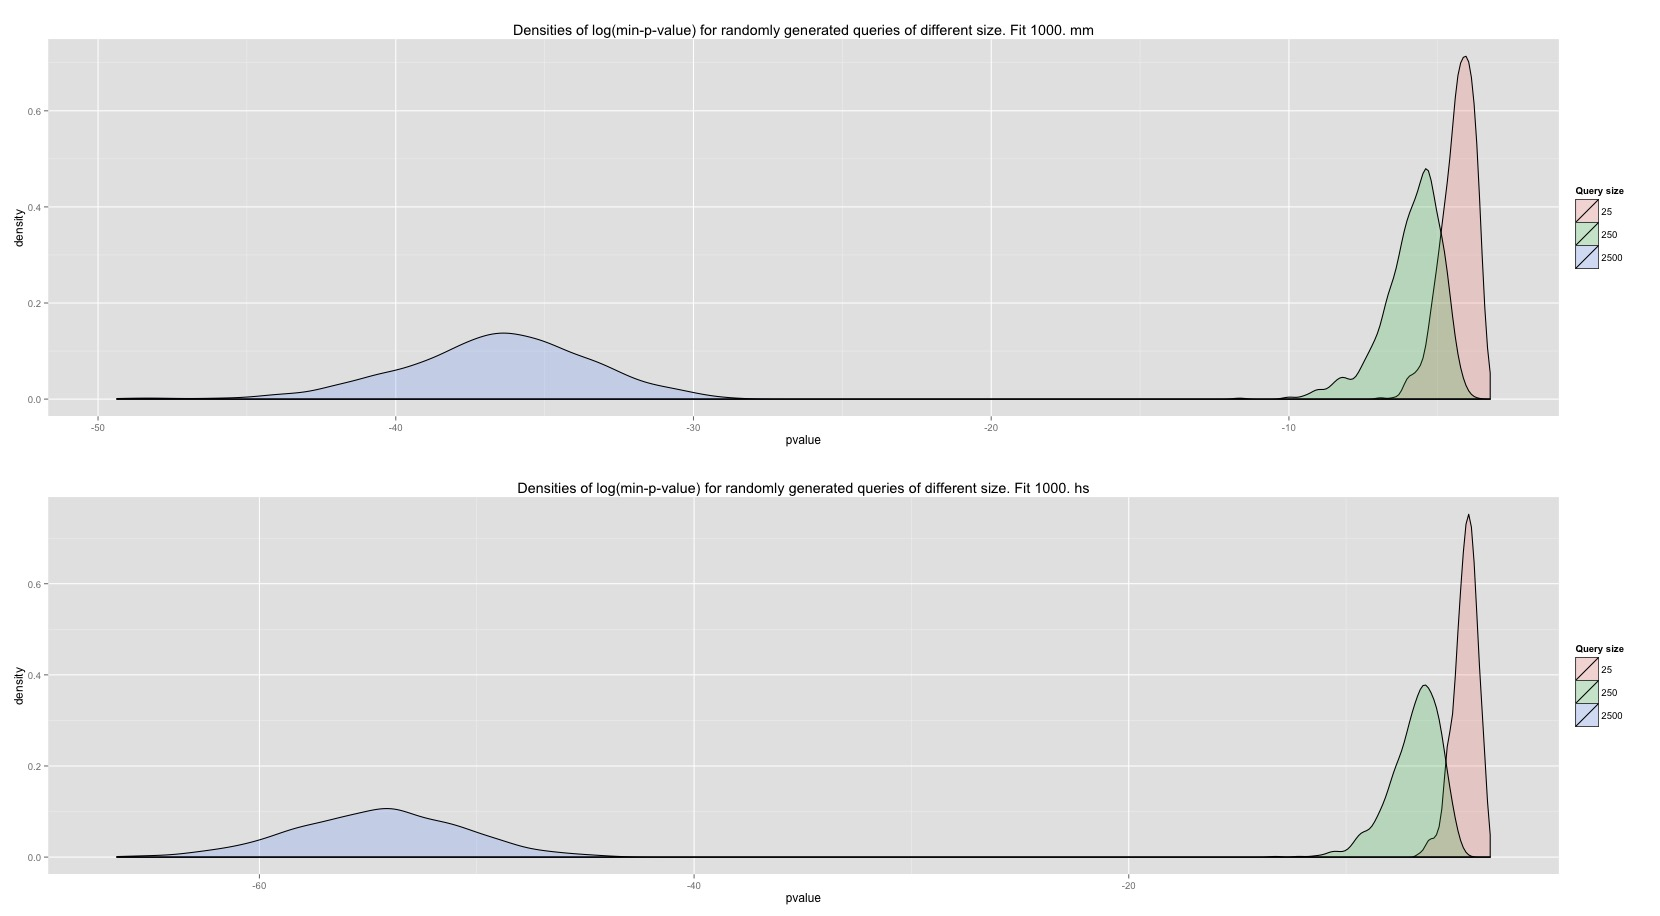
\includegraphics[width=\textwidth]{./img/densities_size_25_25_2500_fit_1000.jpeg}
    \end{figure}
\end{frame}

\begin{frame}
    \begin{figure}[!ht]
        \centering
        \caption{Регрессия $mean(log(p_{value}))$ от длины запроса.}
        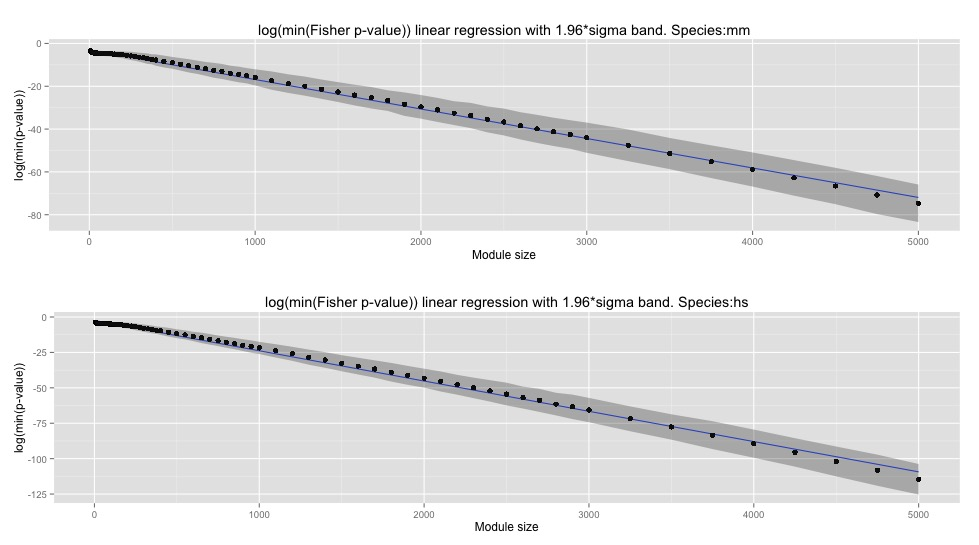
\includegraphics[width=\textwidth]{./img/mean_linear_regression_with_confidence.jpeg}
    \end{figure}
\end{frame}

\begin{frame}{Adjusted $p_{value}$}
  \begin{itemize}[<+->]
    \item Пусть поступил запрос длины $n$, и для всех модулей вычислена значимость $p_i$
    \item Из уравнений регрессий получим значения $mean$ и $std$
    \item Построим нормальное распределение $\mathcal{N}(mean, std)$
    \item Для каждого $p_i$ посчитаем $p^{adj}_i = CDF(p_i) = \mathsf{Pr}(X \le p_i)$ 
        \begin{figure}[!ht]
        \centering
        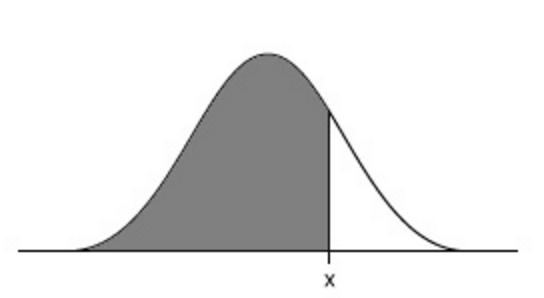
\includegraphics[width=0.4\textwidth]{./img/bell.png}
    \end{figure}
  \end{itemize}
\end{frame}

\begin{frame}{Формирование выдачи}
  \begin{itemize}[<+->]
    \item Оставим только те модули, для которых $p^{adj} \le 0.01$
    \item Отсортируем модули по возрастанию $log(p^{adj})$
        \begin{figure}[!ht]
            \centering
            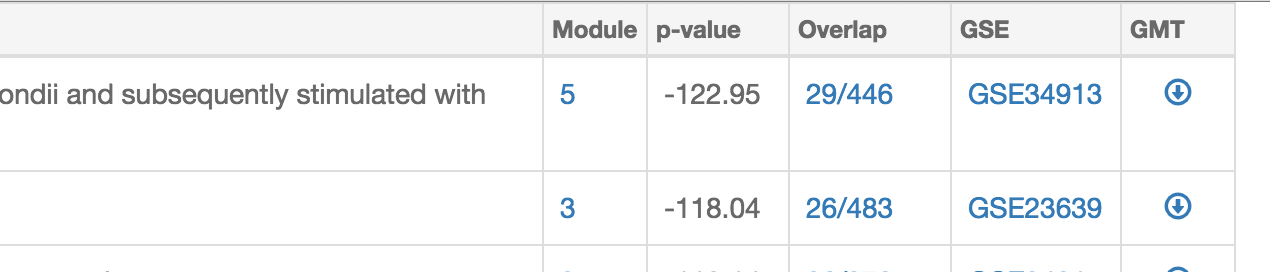
\includegraphics[width=\textwidth]{./img/screen_p_value.png}
        \end{figure}
  \end{itemize}
\end{frame}

\subsection{Тонкости реализации}

\begin{frame}{Общая информация}
  \begin{itemize}[<+->]
    \item Веб-сервис реализован на Python/Django/ReactJS/Java
    \item PostreSQL
    \item Ресурсоемкие вычисления происходят на Java
  \end{itemize}
\end{frame}

\begin{frame}{Скорость вычислений}
  \begin{itemize}[<+->]
    \item Обработка запроса $=$ нахождение $\sim$ 50k пересечений запроса размера $n$ с каждым модулем размера $m_i$
    \item Нужны \emph{все} модули для вычисления результата
    \item Считывание всех модулей каждый раз из БД --- долго (около 40 сек на запрос) и нагружает БД
  \end{itemize}
\end{frame}

\begin{frame}{Оптимизации}
  \begin{itemize}[<+->]
    \item Вычислительный сервер на Java
    \item Храним данные в оперативной памяти
    \item Используем примитивные типы данных: \sout{List<Double>} double[]
    \item Храним модули отсортированными, чтобы пересекать их с запросом за $O(\mathsf{min}(m_i, n))$
    \item Профит! ($\sim$ 3 сек на запрос)
  \end{itemize}
\end{frame}


\section{Уточнение модели}

\begin{frame}{Все плохо}
  \begin{itemize}[<+->]
    \item описать, как все плохо
  \end{itemize}
\end{frame}

\section{Аннотация генов}
\section{Ортология}



\begin{frame}[fragile]
  \frametitle{mtheme}

  The \textsc{Metropolis} theme is a Beamer theme with minimal visual noise
  inspired by the \href{https://github.com/hsrmbeamertheme/hsrmbeamertheme}{\textsc{hsrm} Beamer
  Theme} by Benjamin Weiss.

  Enable the theme by loading

  \begin{verbatim}    \documentclass{beamer}
    \usetheme{m}\end{verbatim}

  Note, that you have to have Mozilla's \emph{Fira Sans} font and XeTeX
  installed to enjoy this wonderful typography.
\end{frame}
\begin{frame}[fragile]
  \frametitle{Sections}
  Sections group slides of the same topic

  \begin{verbatim}    \section{Elements}\end{verbatim}

  for which \textsc{Metropolis} provides a nice progress indicator \ldots
\end{frame}

\section{Elements}

\begin{frame}[fragile]
  \frametitle{Typography}
      \begin{verbatim}The theme provides sensible defaults to
\emph{emphasize} text, \alert{accent} parts
or show \textbf{bold} results.\end{verbatim}

  \begin{center}becomes\end{center}

  The theme provides sensible defaults to \emph{emphasize} text,
  \alert{accent} parts or show \textbf{bold} results.
\end{frame}
\begin{frame}{Lists}
  \begin{columns}[T,onlytextwidth]
    \column{0.33\textwidth}
      Items
      \begin{itemize}
        \item Milk \item Eggs \item Potatos
      \end{itemize}

    \column{0.33\textwidth}
      Enumerations
      \begin{enumerate}
        \item First, \item Second and \item Last.
      \end{enumerate}

    \column{0.33\textwidth}
      Descriptions
      \begin{description}
        \item[PowerPoint] Meeh. \item[Beamer] Yeeeha.
      \end{description}
  \end{columns}
\end{frame}
\begin{frame}{Animation}
  \begin{itemize}[<+- | alert@+>]
    \item \alert<4>{This is\only<4>{ really} important}
    \item Now this
    \item And now this
  \end{itemize}
\end{frame}
\begin{frame}{Figures}
  \begin{figure}
    \newcounter{density}
    \setcounter{density}{20}
    \begin{tikzpicture}
      \def\couleur{alerted text.fg}
      \path[coordinate] (0,0)  coordinate(A)
                  ++( 90:5cm) coordinate(B)
                  ++(0:5cm) coordinate(C)
                  ++(-90:5cm) coordinate(D);
      \draw[fill=\couleur!\thedensity] (A) -- (B) -- (C) --(D) -- cycle;
      \foreach \x in {1,...,40}{%
          \pgfmathsetcounter{density}{\thedensity+20}
          \setcounter{density}{\thedensity}
          \path[coordinate] coordinate(X) at (A){};
          \path[coordinate] (A) -- (B) coordinate[pos=.10](A)
                              -- (C) coordinate[pos=.10](B)
                              -- (D) coordinate[pos=.10](C)
                              -- (X) coordinate[pos=.10](D);
          \draw[fill=\couleur!\thedensity] (A)--(B)--(C)-- (D) -- cycle;
      }
    \end{tikzpicture}
    \caption{Rotated square from
    \href{http://www.texample.net/tikz/examples/rotated-polygons/}{texample.net}.}
  \end{figure}
\end{frame}
\begin{frame}{Tables}
  \begin{table}
    \caption{Largest cities in the world (source: Wikipedia)}
    \begin{tabular}{lr}
      \toprule
      City & Population\\
      \midrule
      Mexico City & 20,116,842\\
      Shanghai & 19,210,000\\
      Peking & 15,796,450\\
      Istanbul & 14,160,467\\
      \bottomrule
    \end{tabular}
  \end{table}
\end{frame}
\begin{frame}{Blocks}
  Three different block environments are pre-defined and may be styled with an
  optional background color.

  \begin{columns}[T,onlytextwidth]
    \column{0.5\textwidth}
      \begin{block}{Default}
        Block content.
      \end{block}

      \begin{alertblock}{Alert}
        Block content.
      \end{alertblock}

      \begin{exampleblock}{Example}
        Block content.
      \end{exampleblock}

    \column{0.5\textwidth}

      \metroset{block=fill}

      \begin{block}{Default}
        Block content.
      \end{block}

      \begin{alertblock}{Alert}
        Block content.
      \end{alertblock}

      \begin{exampleblock}{Example}
        Block content.
      \end{exampleblock}

  \end{columns}
\end{frame}
\begin{frame}{Math}
  \begin{equation*}
    e = \lim_{n\to \infty} \left(1 + \frac{1}{n}\right)^n
  \end{equation*}
\end{frame}
\begin{frame}{Line plots}
  \begin{figure}
    \begin{tikzpicture}
      \begin{axis}[
        mlineplot,
        width=0.9\textwidth,
        height=6cm,
      ]

        \addplot {sin(deg(x))};
        \addplot+[samples=100] {sin(deg(2*x))};

      \end{axis}
    \end{tikzpicture}
  \end{figure}
\end{frame}
\begin{frame}{Bar charts}
  \begin{figure}
    \begin{tikzpicture}
      \begin{axis}[
        mbarplot,
        xlabel={Foo},
        ylabel={Bar},
        width=0.9\textwidth,
        height=6cm,
      ]

      \addplot plot coordinates {(1, 20) (2, 25) (3, 22.4) (4, 12.4)};
      \addplot plot coordinates {(1, 18) (2, 24) (3, 23.5) (4, 13.2)};
      \addplot plot coordinates {(1, 10) (2, 19) (3, 25) (4, 15.2)};

      \legend{lorem, ipsum, dolor}

      \end{axis}
    \end{tikzpicture}
  \end{figure}
\end{frame}
\begin{frame}{Quotes}
  \begin{quote}
    Veni, Vidi, Vici
  \end{quote}
\end{frame}

\begin{frame}{References}
  Some references to showcase [allowframebreaks] \cite{knuth92,ConcreteMath,Simpson,Er01,greenwade93}
\end{frame}

\section{Conclusion}

\begin{frame}{Summary}

  Get the source of this theme and the demo presentation from

  \begin{center}\url{github.com/matze/mtheme}\end{center}

  The theme \emph{itself} is licensed under a
  \href{http://creativecommons.org/licenses/by-sa/4.0/}{Creative Commons
  Attribution-ShareAlike 4.0 International License}.

  \begin{center}\ccbysa\end{center}

\end{frame}

\plain{Questions?}

\begin{frame}[allowframebreaks]

  \frametitle{References}

  \bibliography{demo}
  \bibliographystyle{abbrv}

\end{frame}

\end{document}
